% The \documentclass command is the first command in a LaTeX file.
\documentclass{bsu-ms}
%\documentclass[project]{bsu-ms}  % for project reports

% "bsu-ms" is our "in-house" class file for Boise State theses and project
% reports.


%%%%%%%%%%%%%%%%%%%%%%%%%%%%%%%%%%%%%%%%%%%%%%%%%%%%%%%%%%%%%%%%%%%%%%%%%%%%%%
% Some General Information about LaTeX
%
% LaTeX source (also called "code") files are split into two basic parts:
% the preamble, which contains package loading commands, and other
% document-wide definitions, and the main document text.  The preamble starts
% with the \documentclass command and ends with the \begin{document} command.
% The main text is contained between the \begin{document} and \end{document}
% commands.  
%
% Only LaTeX commands (and whitespace) are allowed in the preamble.  A LaTeX
% command has the form
%
%   \<name>{<arg>}{<arg>}...
%
% where the number of arguments is set by the command definition. 
% Some commands allow an optional argument
%
%   \name[<opt>]{<arg>}{<arg>}...
%
% which may or may not be given.  There are also LaTeX environments
%
%   \begin{<name>}...\end{<name>}
%
% which can be nested, but must be balanced. 
%
% (If you haven't already guessed, anything after a '%' character on a line
% is taken as a comment and ignored.)
%
% In the main text all non-commands and non-comments are treated as ordinary 
% text.  LaTeX normally treats any run of spaces as a single space.  Line 
% breaks are ignored (TeX uses its own linebreaking algorithm); blank lines
% are paragraph separators.  Runs of blank lines are treated as a single
% blank line.  A common mistake novice users make is to try to use literal
% spacing and line breaks in the .tex file to control formatting.  

%%%%%%%%%%%%%%%%%%%%%%%%%%%%%%%%%%%%%%%%%%%%%%%%%%%%%%%%%%%%%%%%%%%%%%%%%%%%%%
% Packages

% The 'graphicx' package is quite extensive; the main purpose here is
% the includion of PostScript graphics.  The 'dvips' option makes it work
% better with 'dvips' (which is what is often used under Linux)
%\usepackage[dvips]{graphicx}
% Comment the above line and uncomment below to use pdflatex
\usepackage[pdftex]{graphicx}
% Then the figures should be in pdf, jpg or png format.
\usepackage{setspace}
\usepackage{xspace}
% The hyperref package provides support for hyperlinks inside/outside the document
\usepackage{url}
%\usepackage[colorlinks=true]{hyperref}
\usepackage{multirow}
 \usepackage{graphicx}
  \usepackage{comment}
  \usepackage{color}
% Others to consider

% The 'subfigure' package does a nice job handling and labelling subfigures
%\usepackage{subfig}

% If you want to use PostScript fonts (or the Nimbus knockoffs) try
%\usepackage{mathptmx}
%\usepackage[scaled=0.92]{helvet}

% The 'citesort' package puts mutliple citation numbers in order
%\usepackage{citesort}


% Generate intra-document links and also allows url and href commands for
% to generate embedded links in the document.
% This breaks the build right now :-(
%\usepackage{hyperref}
%\hypersetup{
%	colorlinks=true
%}


%%%%%%%%%%%%%%%%%%%%%%%%%%%%%%%%%%%%%%%%%%%%%%%%%%%%%%%%%%%%%%%%%%%%%%%%%%%%%%
% Local commands

% Define your macros (new commands) here.


%%%%%%%%%%%%%%%%%%%%%%%%%%%%%%%%%%%%%%%%%%%%%%%%%%%%%%%%%%%%%%%%%%%%%%%%%%%%%%
% Front Matter Definitions
%%%%%%%%%%%%%%%%%%%%%%%%%%%%%%%%%%%%%%%%%%%%%%%%%%%%%%%%%%%%%%%%%%%%%%%%%%%%%%

% These definitions are used by the commands below to construct the front 
% matter pages.  

% Document title
% The \titleBreak command produces a line break in the title on the
% title page (this may be necessary to keep longer titles from looking
% strange)
\title{Towards Multilingual Readability Assessment}  

% Author's name (must be exactly what name the Registrar has)
% normally it is of the form "First Middle Last"
\author{Ion Madrazo Azpiazu}  

% Day of oral defense
\graduationDay{1st}

% Month of graduation (do not abbreviate)
\graduationMonth{December}

% Year of graduation
\graduationYear{2014} 

% Advisor (chair) 
% Use full name, with surname last, without any titles
% The \advisor command accepts an optional argument that specifies the
% advisor's position, which defaults to "Advisor"; for example,
%
% \advisor[Chair]{Foo the Great} 
%
% causes "Chair" to appear on the approval page (the one with the signatures) 
% in place of "Advisor"
\advisor{Sole Pera, Ph.D.} % also the chair of your committee

% Committee members: \committeeA is listed first after the advisor,
% \committeeB second, etc.  An optional argument is accepted to replace
% the default "Committee Member" position.
\committeeA{Tim Andersen, Ph.D.} 
\committeeB{Nere Lete, Ph.D.}

% Master's committees normally have three members, but in case there is
% a need for more, use these commands
%\committeeC[Ex-Officio Committee Member]{ccc}
%\committeeD{ddd}

% Full name of the degree; normally "Master of Science"
\degree{Master of Science}

% Full name of major
\major{Computer Science}

% Major department
\department{Computer Science}

% College 
\college{Engineering}

% Current department chair (at the moment, this is not used)
\departmentChair{Tim Andersen}

% Current graduate dean
\graduateDean{John R. Pelton}

\newcommand{\projectName}{MRAS\xspace}


% Document abstract
\abstract{ An \emph{abstract} is a brief summary of the document.  A typical
  abstract provides a brief introduction, enough to provide context for the
  document, explains the purpose of the thesis or project, and summarizes the
  major results and conclusions.  Keep in mind that a casual observer is
  likely to judge the content of the document by the abstract and title alone.
  (There is an old addage: ``in a joke, the punchline comes at the end; in a
  paper [or thesis], it comes in the abstract.'')  A single concise paragraph
  usually suffices for the abstract.  If it spills onto a second page, it is
  probably too long.  }


% The remaining elements are optional

% \includeCopyright causes a copyright page to be produced.  It is not
% required; in fact, a copyright notice is no longer needed to ensure
% copyright protection.  
\includeCopyright

% \maxPage is used to format the page numbers in the table of contents.
% The actual value is not important: the width of the value given is used
% as the maximum width of any page number.  The following values are suggested
%
% \maxPage{99} for less than 100 pages (this is the default)
% \maxPage{199} for less than 200 pages
% \maxPage{999} for less than 1000 pages 
%
% (If the work is more than 1000 pages, consider cutting it down!)
% The space has to be wide enough for front matter page numbers, which are
% miniscule Roman numerals.  This might have to be widened if there are
% more than 12 front matter pages (which might happen if there is a long
% list of symbols or list of abbreviations, like this template has).
\maxPage{199}

% The Acknowledgments page is a place for the author to express thanks
% or generally acknowledge anyone or anything that assisted in the 
% project or research.  If the student was supported even in part by 
% funding from research grant, it needs to be acknowledged here.
% The Acknowledgments section can have multiple pages, just like the
% Abstract section, but like the abstract, more than one page is probably
% too long.  Acknowledgments are often written in the third person, but
% it is one place (the only place) in the document where first-person
% references (i.e., the use of "I") can be acceptable.
\acknowledgments{
The author wishes to express gratitude to Foo.  This work would have been
partially supported by some particular grant, if there was one.
}
% Hiru hizkuntzatan

% The work can be "dedicated" to someone, typically family members or
% someone similar.  Unlike acknowledgments, which are included in almost
% every thesis or prject, many students omit the dedication.
%\dedication{dedicated to foo}


% A brief autobiographical sketch can be included.  Many students omit this.
% If it is included, remember that it is a sketch, so keep it brief.  Also
% try to limit the content to academically relevant material, such as under-
% graduate work, previous graduate work, employment, etc.  Some students
% like to include their military service.  Otherwise, unless you have
% overcome some particular adversity, it's probably better to leave out
% personal information.
%\biosketch{
%Foo Admirer was born admiring Foo. Foo Admirer has been %tinkering
%with admiration of Foo for a long time. Now it is time to %to be blessed by
%Foo.
%}

% The title of the bibliography defaults to "References" but if you include
% references that are not specifically cited in the text, it needs to be
% titled "Bibliography" instead.
%\bibliographyName{Bibliography}


% (End of preamble)
%%%%%%%%%%%%%%%%%%%%%%%%%%%%%%%%%%%%%%%%%%%%%%%%%%%%%%%%%%%%%%%%%%%%%%%%%%%%%%



% \begin{document} begins the document text, including front matter material

\begin{document}

% The \frontmatter command prepares for front matter material
\frontmatter  %! Do not remove! 

% The \buildFrontPages builds all the front matter pages
\buildFrontPages %! Do not remove! 

% The (optional) list of abbreviations goes here
\begin{listAbbreviations}
  \item[IR] Information Retrieval
  \item[NLP] Natural Language Processing
  \item[PoS] Part of Speech
\end{listAbbreviations}


% The (optional) list of symbols goes here
\begin{listSymbols}
  \item[$\sqrt{2}$] square root of 2
  \item[$\lambda$] lambda symbol, normally used in lambda calculus but
    it sometimes gets used for wavelength as well
\end{listSymbols}


% The main text of the work starts here.  The first chapter is normally
% named "Introduction".

\mainmatter

% Note that judiciously placed comments can serve as landmarks, just as
% in program source code.

%%%%%%%%%%%%%%%%%%%%%%%%%%%%%%%%%%%%%%%%%%%%%%%%%%%%%%%%%%%%%%%%%%%%%%%%%%%%%%
%
% Chapter: Introduction
%
%%%%%%%%%%%%%%%%%%%%%%%%%%%%%%%%%%%%%%%%%%%%%%%%%%%%%%%%%%%%%%%%%%%%%%%%%%%%%%

\chapter{Introduction}

%context, audience (who cares)
%flow with existing measures
%high level satement of need)
% 	multilingual
%	multidomain(twitter, short, long)
%	mltipurpose
%MRAS overview, sell, novelty, contribution




Reading is an important skill in the academic environment, a competence that can be critical for students' educational opportunities and their careers \cite{robinson2000issues}. As reported by Lennon and Burdick \cite{lennon2004lexile}  reading for learning takes place when the reader comprehends  75\% of a text. This represents an appropriate balance that allows the reader to positively understand the text, while also finding challenges in the reading process that will motivate  him to improve his skills \cite{lennon2004lexile}. Outside the educational environment, reading generally takes place for comprehension rather than for learning. In this context, it is critical to provide people with texts they can fully understand. For example, patients 
that properly understand documents disclosed to them before surgery, are known to be less anxious before the operation and obtain more satisfactory results during posterior treatment \cite{medicalReadability2}. However, recent studies\cite{medicalReadability1,medicalReadability2,medicalReadability3}  show that even medical documents that are supposed to be suited for average readers, tend to be too specialized and even well-educated adults have trouble understanding them.
Whether for learning or understanding, the complexity of texts to be read needs to be determined.


Every reader has different reading skills and the levels of difficulty of the texts they need depends also upon their personal objective. Therefore, providing institutions and readers with tools that can measure the complexity of a text so that they can assess whether it is adequate for a user is imperative. \textit{Readability Assessment (RA)} tools \footnote{RA tool and RA formula are used interchangeably in this document.}  are certainly aimed for handling such a task by providing a mean to determine the degree of ease with which a reader can understand a given text, i.e. the \textit{Readability Score (RS)} of the text.



 Historically, teachers have been the main stakeholders of RA formulas, using them to select new materials for their courses and curriculum design. However, lately, more stakeholders have found benefits in using RA tools outside the academic environment. Automatic text simplification\cite{textsimplification1,textsimplification2}, summarization for people with reading difficulties\cite{textsimplificationWithDisabilities1}, book recommendation \cite{pera2014automating}, literacy assessment\cite{literacy1}, or legal and medical document complexity assessment\cite{medicalReadability1,legalreadability,medicalReadability2,medicalReadability3}  are only a few examples of applications that take advantage of the complexity levels generated by existing RA tools. Even in commercial environments, book publishers require professional linguistic services in order to tag their publications with a readability level required for their intended audience, a task that could similarly be completed by an automatic tool.

In estimating the complexity of texts, traditional formulas, such as Flesh \cite{flesch1948new}, became very popular in the late 1940's among educators for manually determining text difficulty. Most of these formulas relied on \textit{shallow features}, which could easily be adapted to multiple languages and provide a simple way of determining text complexity. The multilingualism achieved by traditional formulas offered numerous benefits in contexts where the readability of more than one language was needed, i.e., book translation or learning a second language. However, traditional formulas were known to lack precision. For example, they could classify nonsense text as \textit{simple to read}, just because it contained short and frequently-used words \cite{davison1982failure}. The insufficient precision encouraged researchers to study and develop better and more sophisticated methods for RA that depended upon more in-depth text analysis \cite{franccois2012ai,aluisio2010readability}. These new formulas continued taking advantage of  shallow  features, but incorporated more complex features based on the syntax and semantics of text. With the addition of new text complexity indicators, the tools became more precise, but at the same time more constrained regarding their language adaptability \cite{benjamin2012reconstructing,feng2010comparison}. In fact, they used increasingly more language-dependent techniques, which made the systems unadaptable to estimate RS for text in languages other than the one they were designed for. As a result, the multilingualism that was possible in the early stages disappeared.  

%Using a multilingual readability assessment tool would suppose multiple benefits to task such as, translation, where the translator (whether a human or a machine) could compare the multiple translations' readability in order to choose the one that best captures to the original text, or book recommendation systems, who would no longer need to use multiple readability assessment tools when dealing with multiple language contents. {\color{red}Any more ideas? }
With multilingualism and precision in mind, we propose to develop \textbf{MRAS}, a \textbf{M}ultilingual \textbf{R}eadability \textbf{A}ssessment \textbf{S}ystem. This tool should both show results comparable to monolingual state-of-the-art systems  and  maintain the multilingualism the early tools in the RA field had. For doing so, we will (1) explore features and methods used in literature, (2) design novel features that positively influence the readability level estimating process and (3) analyze how all those features can be adapted to be used in multilingual RA.
%For doing so we will explore features and methods used in literature and adapt them to be multilingual. Furthermore, we will conceive novel features and analyze the effect each of them has regarding readability. This will also allow us to determine which features determine readability in a text in overall and for specific languages.
MRAS will be \textit{open source} and \textit{easily connected} to different applications that require RA as a service, potentially permitting the analysis of all sorts of texts, including text snippets, books, websites and even short and unstructured texts, such as the ones found in social media. In doing so, we will create a system that will adapt itself to the input text language and use an adequate subset of features for the corresponding language for readability prediction, creating, to the best of our knowledge, the first multilingual readability assessment system.

As a byproduct of our research work, we will create a leveled dataset with readability-labeled documents for different languages, which currently is unavailable. In addition, we will create an in-depth report surveying existing strategies for readability prediction.

It is important to note that, for practical purposes, the proposed application will only be tested in three different languages: \textit{English}, for state of the art comparison purposes and as reference of germanic languages. \textit{Spanish}, as a reference for romance languages, and \textit{Basque} as an example of a pre-indoeuropean and minority language.


\chapter{Related work}

%Update with new refs
%traditional
%state-of-art
%by lang
%compare/contrast along the way
%multipurpose

From the past six decades, different RA systems have been developed with high diversity in terms of both languages and features \cite{feng2010comparison,benjamin2012reconstructing}. Initial readability formulas, such as Flesh \cite{flesch1948new}, Dale-Chall \cite{chall1995readability}, and Gunning FOG \cite{albright1996readability} made use of \textbf{shallow features}, mostly based on ratios of characters, terms, and sentences. These formulas, were basic enough even to be computed manually, providing a simple way of estimating a text's complexity, even if the formulas lacked precision in some cases \cite{davison1982failure}. This simplicity, however, made them easy to be adapted to estimate readability scores in different languages \cite{spaulding1956spanish}.

In recent years, readability formulas have evolved to supervised learning based systems that use a combination of traditional shallow features and new natural language processing based ones, which consider language aspects, such as syntax or semantics of texts. However, incorporating  new features has brought a drawback to the area, evidenced by the fact that current systems are too focused in certain languages, making them only functional in the languages they were created for. Current state-of-the-art is composed by methods focused on specific languages, as discussed below:


For \textbf{English}, 
% various surveys \cite{feng2010comparison,benjamin2012reconstructing} comparing features used in the literature were presented. 
the RA system presented in \cite{aluisio2010readability} predicted only two levels of difficulty, simple or complex, using elaborated features, such as ambiguity among the terms in the texts. Other authors \cite{textsimplificationWithDisabilities1}, oriented their system for assessing the difficulty level of a text for people with intellectual disabilities by developing features that were intended to detect how well a text was structured. A readability prediction system for  finalcial documents was presented in \cite{bonsall2015plain}, which was based on features such as the presence of active voice or number of hidden verbs. It is also important to mention two commercial RA tools, Lexile\footnote{https://www.lexile.com/} and AR \footnote{http://www.renaissance.com/products/accelerated-reader/atos-analyzer}, which are widely used among English speaker academic professionals. Even if their algorithms are not public, they are known to use shallow features showing how common terms of a text are and how long sentences are in average \cite{lennon2004lexile}. The literature pertaining to RA for text in English is abundant. For more in-depth discussion on RA formulas refer to \cite{feng2010comparison,benjamin2012reconstructing}.


In contrast to English, \textbf{Spanish} RA has not seen any significant improvement regarding features in recent years, as most of the existing works are still based on shallow features. Among the well-known RA tools for Spanish,  SSR \cite{spaulding1956spanish} was based on the analysis of sentence length and number of rare words per sentences, whereas LC and SCI \cite{anula2007tipos} were based on density of low frequency words in text. Other systems \cite{vstajner2013readability,drndarevic2013automatic} presented strategies to combine the aforementioned methods to improve RA estimation.





Compared to other languages, \textbf{Basque} RA is reduced to only one system. Due to the fact that Basque is considered a minority language and shares little similarity with most spoken languages, limited research has been done in the area. So far,  ErreXail \cite{gonzalez2014simple} is the only system created for Basque RA. ErreXail was developed to predict two different readability values, simple or complex, using features mostly based on ratios of common natural language processing labels, such as Part-of-Speech tags or morphology annotations.

Similar to Basque, the literature for \textbf{Arabic} RA is limited as well. Al-Ajlan and Al-Khalifa \cite{al2008towards} developed a RA tool based on only two features: average letters per term and average terms per sentence. These, features were analyzed using a Support Vector Machine classifier in order to classify text as simple or complex.

Opposed to RA tools for previous languages, structural features do not seem to have such a success for \textbf{Chinese} RA. Therefore, most of the research works  related to Chinese RA have been focused only on lexical features, such as Tf-Idf of terms \cite{chen2011chinese,collins2004language}.


%The system introduced in \cite{chen2011chinese} was only based on lexical metrics based on the TF-Idf measure. However this technique was not topic independent, as once trained for a certain topic the terms were no longer useful for other ones. Another system \cite{collins2004language} already tried to solve this issue for Chinese. This system was based on Tf-Idf too and as the authors stated, removing some top scoring words of the Tf-Idf ranking, lead the system to be more independent of the topic. 

In contrast to the aforementioned techniques, the authors of \cite{dell2011read}   presented a RA system for \textbf{Italian} aimed at assessing readability at sentence level, which combined traditional, lexical, and syntactical methods.% The developed system was intended to be part of a simplification tool the authors were also developing, which required of a RA system that worked on sentences rather than on full texts.


% Since the text simplification tool the authors were developing was based on sentences, the authors of this system decided that rather than developing a system for determining text readability, their system would work at sentence level. Therefore, the text simplification tool, would have more information of which sentence needed simplification and which did not. The model generated for sentence level was shown to be generalizable to full text level, by the use of simple averages. The more complex sentences a text have, the more probabilities it have to be complex in overall.

Rather than focusing on the general reader,  Fran{\c{c}}ois and Fairon \cite{franccois2012ai} developed a RA system for \textbf{French} with foreign language learners in mind. The objective was to determine which features were more important for a foreign language learner to understand a text. They tested lexical, syntactical and semantic features and showed that semantic ones performed poorly in their case.

% In addition, they provided a metric new to the area called adjacent accuracy that tried to measure systems' performance in a more accurate and relevant way. 



Even if the number of RA systems that tackle individual languages is high, they are usually focused on a specific set of features and materials they can analyze. In addition, to best of our knowledge, none the RA systems presented are \textbf{multilingual}. MRAS will not only be multilingual, but will also be based on a comprehensive set of existing and novel features which will be general enough to potentially be able to handle all sorts of reading materials. All those characteristics will make MRAS a unique system in the area.

%TODO TOASK, I dont like this paragraph


% They are too focused in alangauge
% They focus a certain typeo of material
% None of the uses the whole set of features
% Not multilingual



\chapter{Method}
%overview + figure
%tools
%preporcessing
%basic features
% traditional, morph, synt, lex, sem, struc
%metadata
%social
%fusion, strategy by purpose



\projectName is a readability assessment system capable of automatically predicting the readability level of any given document, being able to handle multiple document types, differing in format, length and language. For doing so \projectName takes advantage of several tools described in section \ref{sec:tools}, as well as various text processing strategies described in \ref{sec:textprocessing}. This chapter also provides an overview of the design of \projectName in section \ref{sec:overview} and further in-depth detail in sections \ref{sec:features} and \ref{sec:fusion}.






\section{Tools}
\label{sec:tools}

Whether for text processing or for feature extraction, \projectName takes advantage of several existing tools and techniques, which we describe below.

\subsection{NLP Toolkits}
For developing \projectName we analysed several NLP toolkits available in he market.
%TODO Create a table of all the ones analyzed





\subsubsection*{Freeling NLP}
Freeling \cite{padro12,padro10b} is a NLP tookit developed for the easing various natural language analysis tasks. Freeling includes, but is not limited to, tokenization, PoS tagging, syntactic parsing, dependency parsing and semantic labelling. Furthermore, Freeling is, to the best of our knowledge, the only tool kit supporting 14 languages with this depth of analysis, supporting Asturian (as), Catalan (ca), German (de), English (en),  French (fr), Galician (gl), Croatian (hr), Italian (it), Norwegian (nb), Portuguese (pt), Russian (ru), Slovene (sl), Spanish (es), and Welsh (cy).
%\subsubsection*{Latent Semantic Analysis}


\subsection*{SyntaxNet}
%TODO do we use this?
%http://universaldependencies.org/
{\color{red} should I mention why not this one?}


\subsection*{Katea}
Katea is set of NLP tools developed for Basque. Katea is composed by Morpheus \cite{morpheus} (morpho-syntactic analysis), eustagger \cite{eustagger} (lemmatization and syntactic function indentification), eihera \cite{eihera} (named entity detection), ixati \cite{morpheus} (shallow parsing) and maltixa \cite{maltixa} (dependency parsing).






\subsection{WordNet}
Wordnet \cite{miller1995wordnet} is a lexical database for English where terms, i.e., nouns, verbs and adjectives, are grouped into sets of synonyms, expressing different concepts. These concepts are related by each other by several semantic relationships, such as hyperonymie or hyponimie. An example of this structure can be seen in figure \ref{fig:wordnet}, where \emph{motor vehicle} has \emph{vehicle} as hypernym and \emph{car} and \emph{truck} as hyponyms. Note that this structure forms a tree. This fact will be used later, for building some features.




\begin{figure}[h!]
\centering
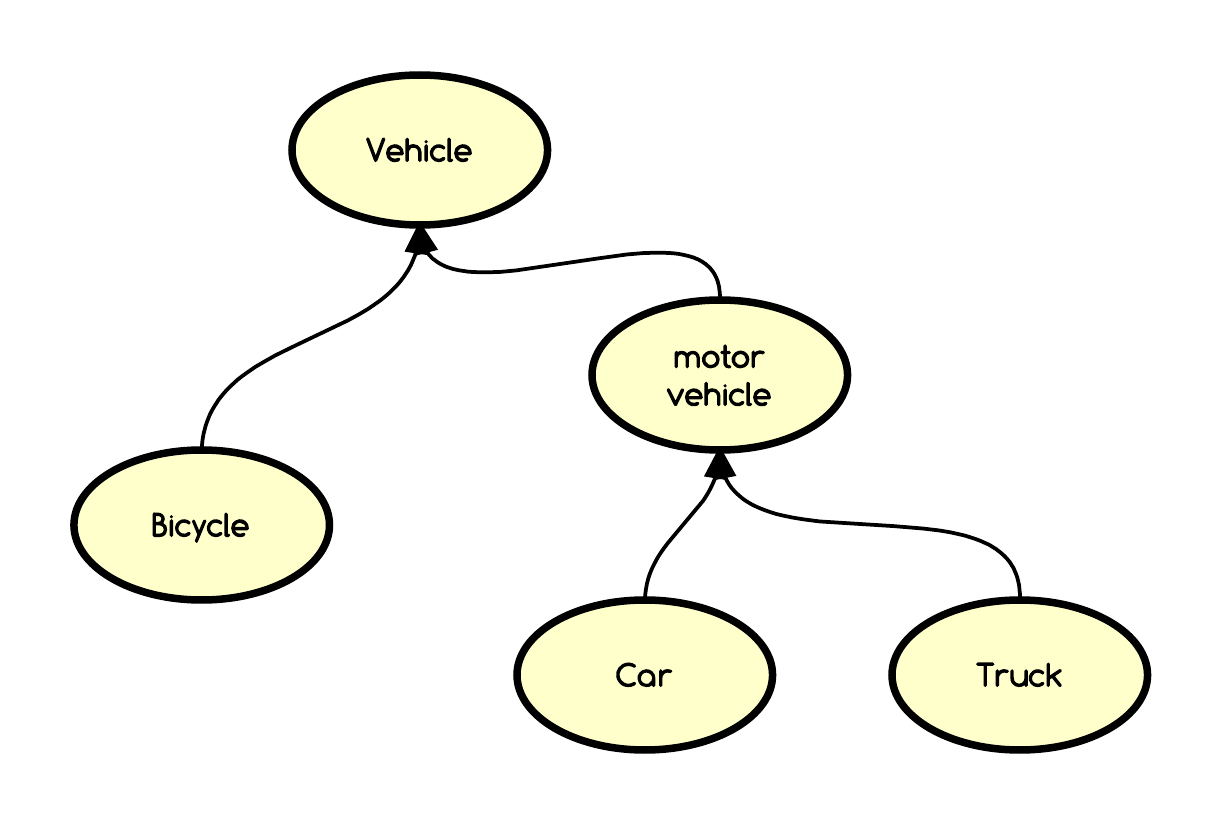
\includegraphics[width=0.7\textwidth]{wordnet}
\caption{Wordnet example}
\label{fig:wordnet}
\end{figure}






\section{Text processing}
\label{sec:textprocessing}
The preprocessing step is the one that takes place first for any document handled by \projectName . The aim of preprocessing is to identify the document to decide further process \projectName needs to perform over it, and to prepare the document for future feature extraction. More detail of mentioned processes is given below.

\subsection{Document type detection}
One of the main features of \projectName is its versatility, since \projectName is capable to predict readability values for documents of different format, length and language. Given this variety of documents, each of them cannot be treated the same way, different strategies need to be applied for different texts. Therefore, each document used by \projectName  is classified using 3 criteria: format, length and language.


{\color{red} should we go deeper? explain how each criteria is determined?}


\subsection{Tokenization}
Tokenization is the process of splitting a text into smaller parts, i.e. tokens. A token represents each sensical part of a text, which usually corresponds to a term, a number, or a punctuation mark. However, sometimes tokens can be formed by a combination of the previous, i.e., \emph{aren't} or \emph{people's}. An example of how a sentence is tokenized can be seen in Table \ref{tab:tokenization}.

\begin{table}[h]
\centering
\begin{tabular}{|l|l|l|l|l|l|}
\hline
\multicolumn{6}{|l|}{Did they win the olimpics?} \\ \hline
did & they & win & the & olimpics & ? \\ \hline
\end{tabular}
\caption{Tokenization example}
\label{tab:tokenization}
\end{table}

\subsection{Stopping}
Stopping or stopword removal refer to the process of removing stopwords from a text. A stopword is a term that does not add any important information to the task that is performed, usually adding unnecessary noise that hinders valuable information among a document. The frequency of a term is a good indicator for stopwords since, usually the terms that most appear in a text are the ones that less information contain. Some examples of general purpose stopwords are \emph{a}, \emph{the} or \emph{is}, however depending on the domain, terms such as \emph{computer} can also be stopwords given its high frequency. The purpose stopping is usually 2-way, speeding up later processes and noise reduction, and is usually performed without the need of any specific tool, just using a stopword list.



\subsection{Stemming/Lemmatization}
The goal of both stemming and lemmatization is to achieve a normalized version of a term. This normalization, is usually helpful for search and comparison task as it reduced the search space among all the terms. As an example, when computing a metric about the verb \emph{play} it might be interesting to compute it for all its word-forms (\emph{play}, \emph{plays}, \emph{played}). This process is usually simpler if all the word-forms are normalized to one canonical form. Stemming and Lemmatization differ in the way the normalized form is obtained. While lemmatization is able to achieve real canonical form (i.e. lemma) of a word (the one appearing in the dictionary), stemming simply chops common prefixes and suffixes to obtain an approximation of it. When both techniques are available \projectName will use lemmatization over stemming, however, some languages do not have any lemmatization technique available. Freeling will be used for lemmatization in Spanish and English, while katea will serve for the same purpose in Basque.




\subsection{Part of Speech Tagging}
%https://www.ling.upenn.edu/courses/Fall_2003/ling001/penn_treebank_pos.html
Part of Speech Tagging is the process of labelling each token with a tag that represent the function each token has in a sentence. PoS tags usually differ from language to language\footnote{As an example, the Penn Treebank project defines 36 PoS tags for English, which can be seen here https://www.ling.upenn.edu/courses/Fall\_2003/ling001/penn\_treebank\_pos.html}, however, the most predominant tags, such as verb, adjective or noun, exist among all the languages. An example of Part of Speech tagging can be seen in Table \ref{tab:postagging}.



\begin{table}[h]
\centering
\begin{tabular}{|l|l|l|l|l|l|}
\hline
did & they & win & the & olimpics & ? \\ \hline
Verb & Pronoun & Verb & Determiner & Noun & Symbol \\ \hline
\end{tabular}
\caption{Part of Speech tagging example}
\label{tab:postagging}
\end{table}



\subsection{Shallow parsing}
Shallow parsing, also called chunking, refers to the process of grouping tokens into chunks. A chunk consists usually a small phrase of about 1 to 4 terms. Those terms are somehow connected to each other and together express a senseful concept. There are two types of chunks, depending if they express a noun or verb phrase. An example of a shallow parsing of a sentence can be seen in figure \ref{fig:shallow}.

\begin{figure}[h!]
\centering

\includegraphics[width=\textwidth]{shallow}
\caption{Shallow parsing example}
\label{fig:shallow}
\end{figure}



\subsection{Dependency parsing}
Dependency parsing goes further than shallow parsing, determining relationships between tokens rather than just grouping them. Given these relationships, a dependency tree is generated, which usually has a root node representing the main verb of the sentence, which has the subject and objects of the sentence as children. An example of a dependency parsed sentence can be seen in figure \ref{fig:dependency}.

\begin{figure}[h!]
\centering
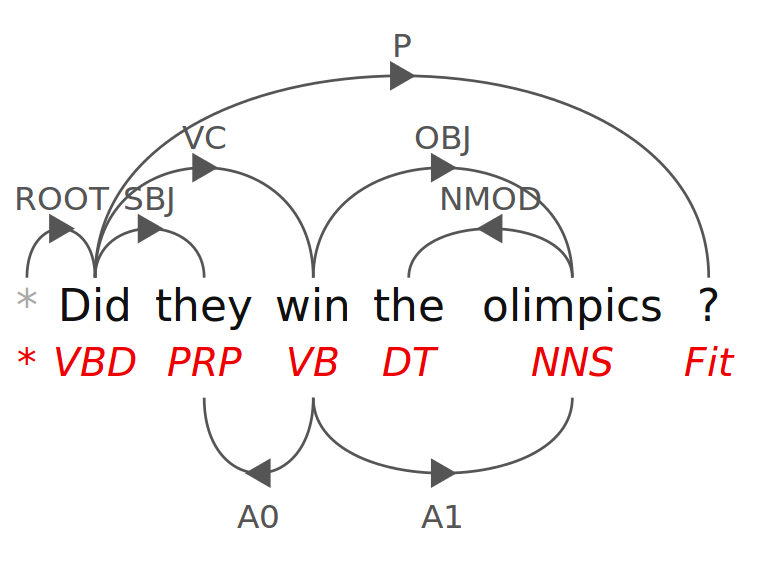
\includegraphics[width=0.8\textwidth]{dependency}
\caption{Dependency parsing example}
\label{fig:dependency}
\end{figure}

\subsection{Named entity detection}
A named entity is a token or group of tokens that represent and known entity such as a person, a location, or an organization. Depending on the complexity of the tool that performs this analysis, those entities can also be linked to a knowledge base such as Dbpedia \cite{dbpedia} where more structured information about the entity can be found.




\begin{table}[h]
\centering
\begin{tabular}{|l|l|l|l|l|l|l|l|l|l|}
\hline
Usain & Bolt & won & the & race & in & Rio & de & Janeiro & . \\ \hline
person & person &   &   &   &   & location & location & location &   \\ \hline
\end{tabular}
\caption{Named entity detection example}
\label{tab:postagging}
\end{table}


\section{Design overview}
\label{sec:overview}





\projectName is based on a supervised learning approach that relies on knowledge acquired from a leveled corpora. In designing \projectName we followed the steps illustrated in Figure \ref{fig:pipeline} and discussed below.



\begin{figure}[h!]
\centering
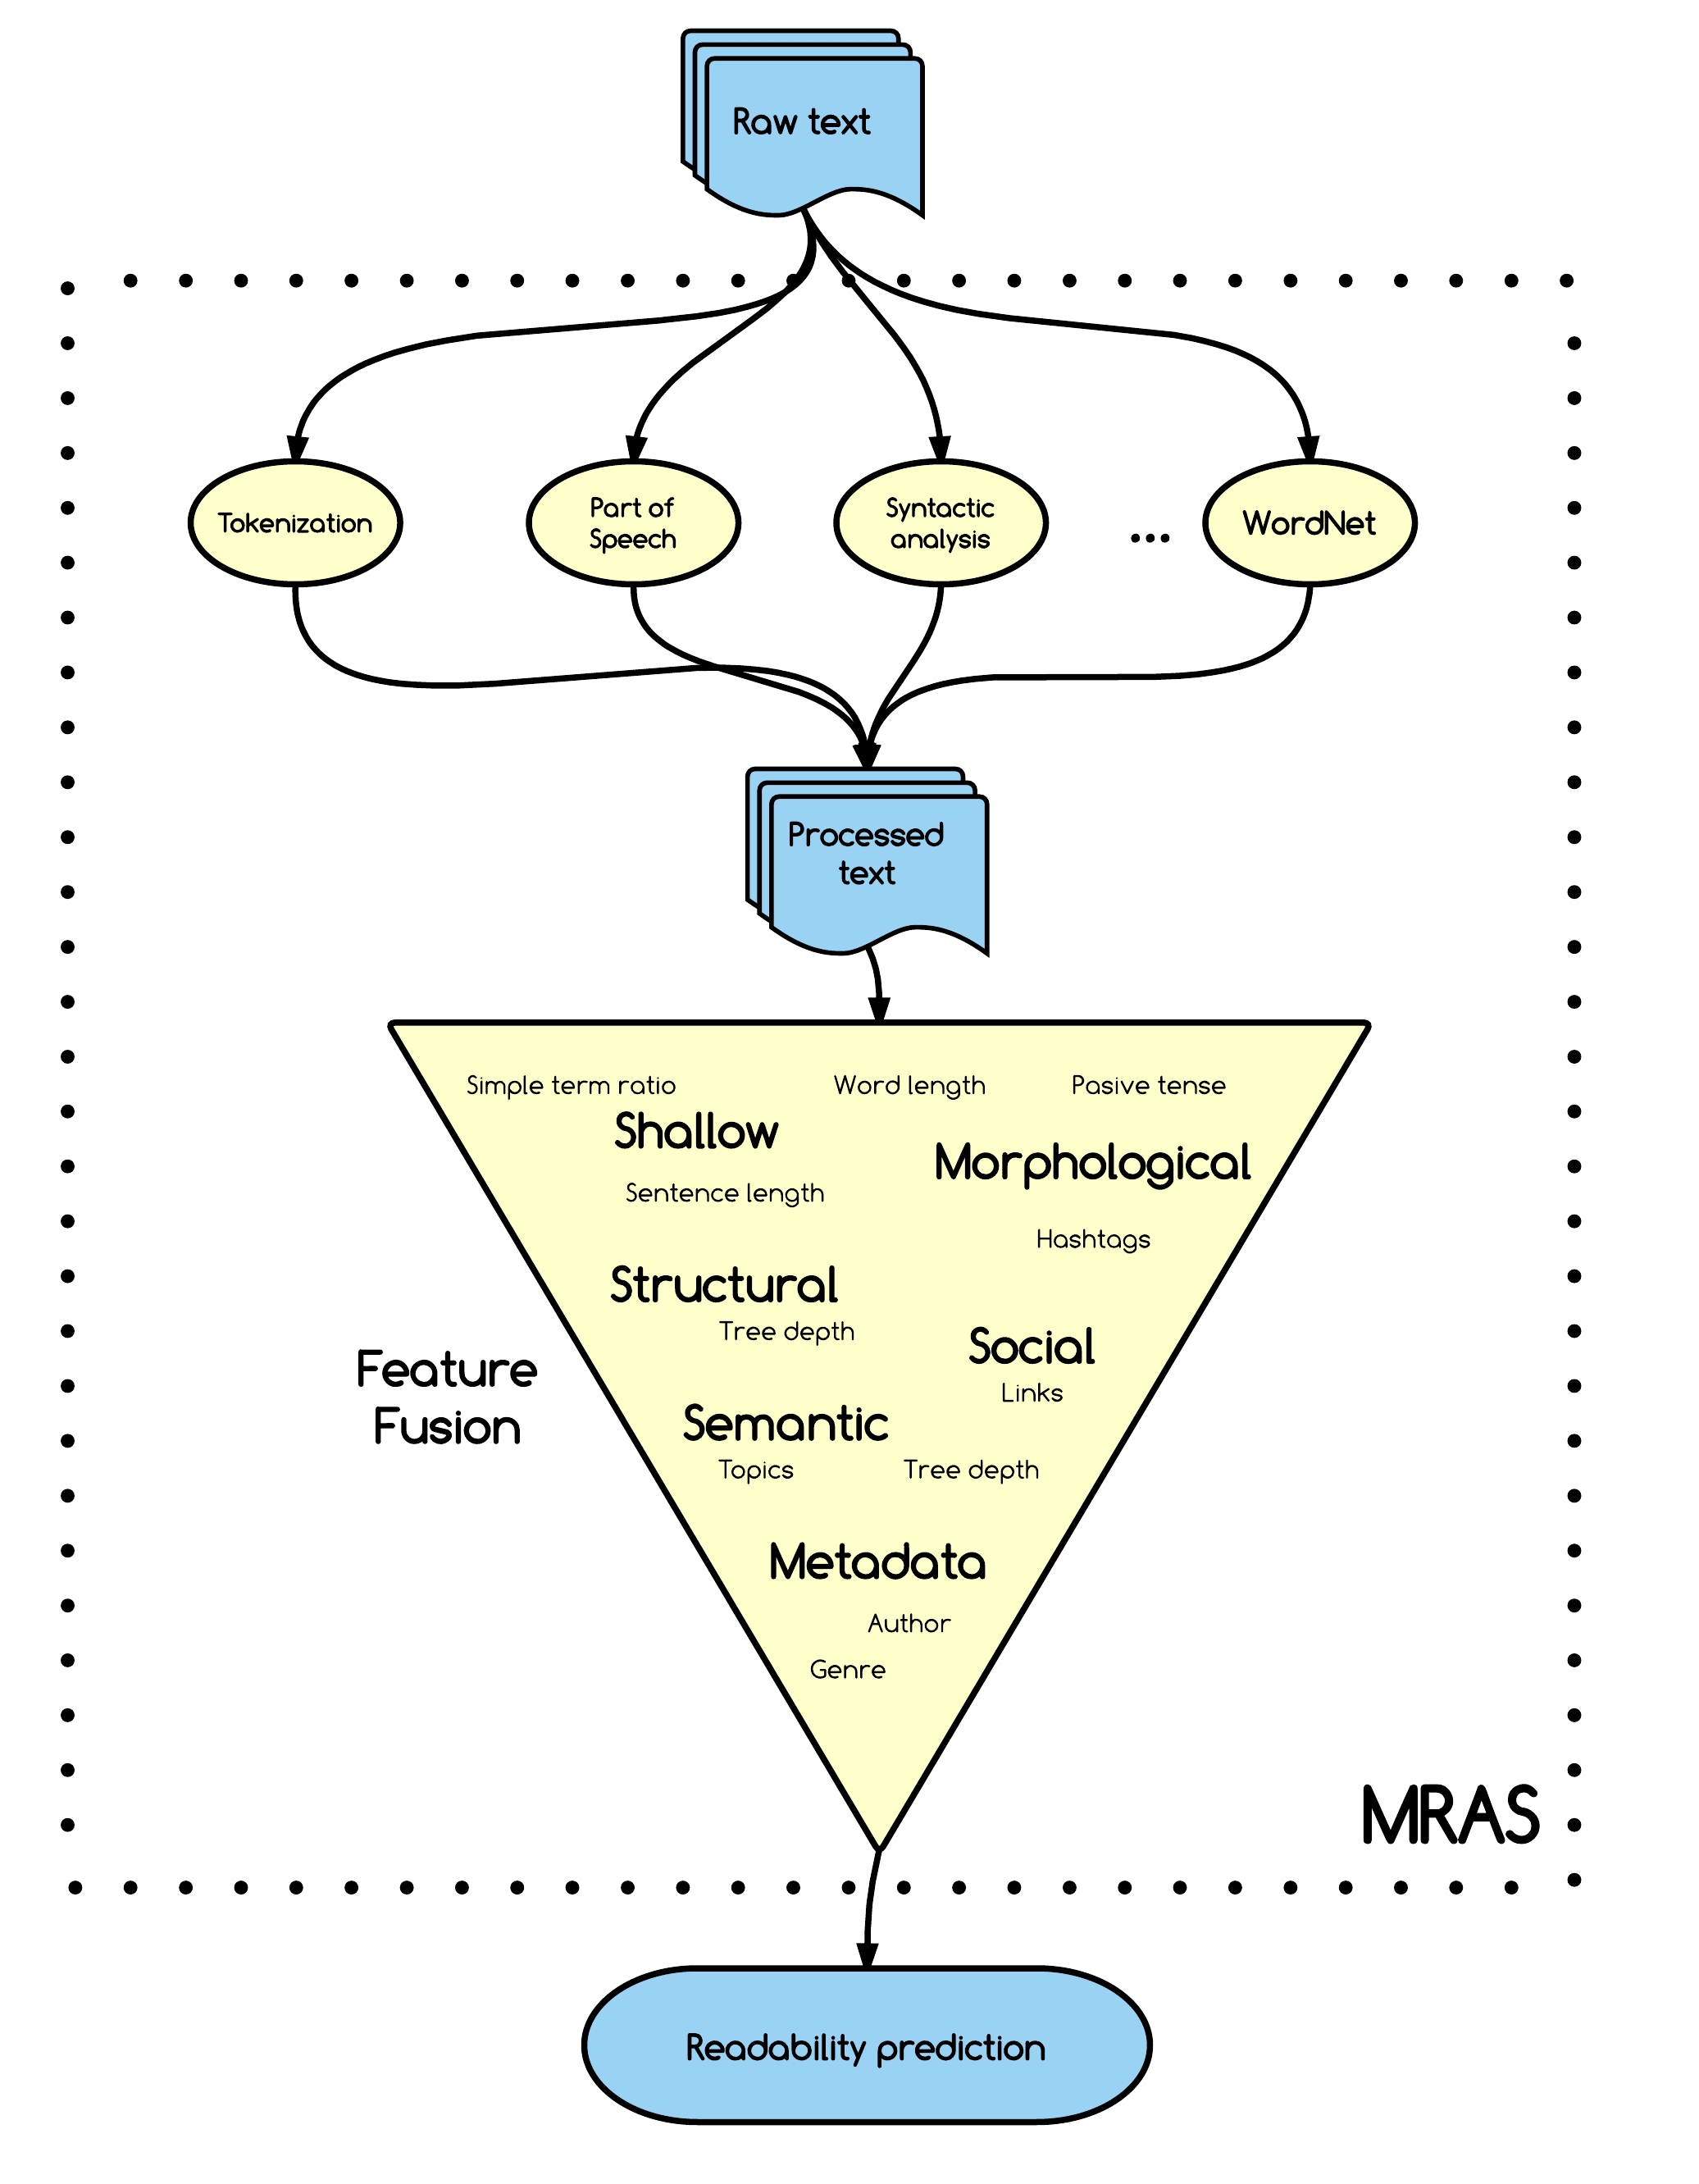
\includegraphics[width=0.8\textwidth]{pipelineGraph}
\caption{\projectName}
\label{fig:pipeline}
\end{figure}



\projectName receives two different inputs: a collection $C$ of documents for each of which a readability label is already assigned, and a document $d$ which its readability is unknown for \projectName and, thus, will be predicted. Both inputs are taken through a preprocessing step described in section \ref{sec:preprocessing}, which cleans, filters and normalizes their content, to prepare them for the feature extraction step described in section \ref{sec:featureExtraction}. These features, serve as a numeric representation for each document. \projectName is capable of learning patterns over the representations extracted from each document in $C$ and use these patters to predict readability scores for new unlabelled documents such as $d$.

















\section{Feature extraction}
\label{sec:features}
Feature engineering is one of the most important aspects of this thesis. A good feature set determines the the quality of a classifier, and therefore the quality of a readability assessment system. A description of each feature included in \projectName is provided below separated in different linguistic levels.


\subsection{Shallow features}

Shallow features \cite{flesch1948new,chall1995readability,albright1996readability} have historically shown to be of good use when predicting readability. Even if they sometimes lack precision \cite{davison1982failure}, they serve as a good baseline for readability assessment systems. A description for each shallow feature is provided below.

\subsubsection*{Word length}
Everyday terms are usually short in most languages, they are preferred for spoken language over their longer analogues, in order to maintain more fluent conversations. In the opposite side, difficult terms are longer the more technical or scientific they are. Therefore, short terms the one youngsters first learn and better comprehend. To take advantage of this fact, \projectName bases 4 features on it,  average length of terms and average length of their lemmas, considering or not stopwords for both cases.



\subsubsection*{Sentence length}
Sentences oriented people with low understanding skill are usually short. They just focus on simple ideas and facts with very simple argumentations. On the opposite side, documents oriented to more technical and complex aspects contain more argumentation and therefore more subclauses in the sentences, resulting in longer sentences. \projectName benefits of this fact generating two features, average word length of sentence with and without stop words.

\subsubsection*{Simple terms}

%TODO






\subsection{Morphological features}
Morphological features capture how terms are formed from their root. Even if this  aspect is not relevant in some languages, such as English, it has been shown to be a strong predictor for readability scores in morphology rich languages such as Basque \cite{gonzalez2014simple}. A description of morphological features included in \projectName is described below.


\subsubsection*{Morphological phenomena frequencies}

\subsubsection*{Inflection ratio}
difference in size between the wordform and the lemma


\subsection{Structural features}
Structural features are the ones that describe how a text is organized. They can both describe structure within the sentence (syntactical structure) or structure between sentences (pragmatical structure). The features that have been implemented in \projectName can be seen below.


\subsubsection*{Structural complexity}
based on a neural network and distributional semantics

\subsection{Semantic features}
Semantic features go beyond the tokens and structure of the text in order to analyse the concepts laying on it.

\subsubsection*{Semantic closeness}
How close is a text from the terms of each group?
Using simple cosine similarity and using the cloud of points created using distributional semantics.
\subsubsection*{Concept densisty}
\subsubsection*{Followability}
\subsubsection*{Ngram frequencies}
\subsection{Social features}
RA can be used in more than just plain text. Internet is evolving into a new social era and so are text resources. Increasingly more resources contain social information, such as hashtags, mentions, or links, a type of information that is usually ignored by readability formulas.

\subsection{Metadata features}
Metadata based features can be useful in environments where text access is limited (i.e. copyrighted material). An exploration of this type of features will also be done in order expand the types of texts MRAS can handle.




\section{Fusioning Strategy}
\label{sec:fusion}












\begin{comment}




\textbf{Morphological features} capture how terms are formed from their root. Even if this  aspect is not relevant in some languages, such as English, it has been shown to be a strong predictor for readability scores in morphology rich languages such as Basque \cite{gonzalez2014simple}. Different morphological phenomena will be analyzed in order to create features in this category.\\

\noindent
\textbf{Structural features} are the ones that describe how a text is organized. They can both describe structure within the sentence (syntactical structure) or structure between sentences (pragmatical structure). Depth of the syntactic tree or ratios of different types of connectors between sentences are some examples of the features that are going to be explored under this category.\\

\noindent
\textbf{Semantic features} go beyond the tokens and structure of the text in order to analyse the concepts laying on it. %This permits to create an abstraction level that leave behind the dependence other features have respect to the text.
 Features such as concept density or concept follow-ability are some examples of the features that will be analyzed under this category.\\

\noindent
RA can be used in more than just plain text. Internet is evolving into a new social era and so are text resources. Increasingly more resources contain \textbf{social information}, such as hashtags, mentions, or links, a type of information that is usually ignored by readability formulas. We propose to investigate how the aforementioned information can be used for readability prediction.

\noindent
\textbf{Metadata} based features can be useful in environments where text access is limited (i.e. copyrighted material). An exploration of this type of features will also be done in order expand the types of texts MRAS can handle.



















\subsection{Text processing}
%MRAS will used leveled corpora for learning from, i.e. a set documents that are labeled for its readability by experts. However, even if those documents are good to read by humans, they cannot be understood by machines, because they contain no structure. Therefore, the first step MRAS will always perform for a text is a processing step, where raw text is given structure and, therefore, value. This structure and information will later be used for extraction features that will help the system predict a readability score.\\
As the main focus of MRAS is to analyze text, we have identified different text processing methods and tools that will be used in its development. \textbf{Freeling NLP} \cite{padro12,padro10b} is a multilingual natural language processing (NLP) toolkit that supports 11 different languages. This tool solves common NLP tasks such as, tokenization, sentence detection, part of speech tagging or dependency parsing. \textbf{WordNet} is a lexical database that takes advantage of semantic relations between terms to build a graph that is very convenient for semantic analysis tasks. \textbf{Latent semantic analysis} is also a commonly used strategy  for semantic analysis, which takes advantage of concurrences among terms for determining similarities between them. All those tools, along with others that we will incorporate during the research process, will be used in the text processing step of MRAS.



%The tool that has been chosen for natural language processing is \textbf{Freeling NLP} \cite{padro12,padro10b}. Freeling is an open source Natural language processing library that supports 11 different languages. The tool solves common NLP tasks that will be used in the processing step, such as, tokenization, sentence detection, Part of speech tagging or dependency parsing. MRAS will also use other tools such as \textbf{WordNet} \cite{miller1995wordnet} or \textbf{Latent semantic analysis} \cite{landauer1998introduction} which will permit the analysis of the text in a semantic way. Each of this processes will be helpful for building certain features later.\\

%The \textbf{tokenization} is the base module for any NLP processing. Tokenization refers to taking a raw text and normalizing it into pieces that make text processing possible. This will also make possible, to implement tradition shallow features such as, Flesch–Kincaid \cite{flesch}. \\

%The \textbf{Part of speech} analysis determines the function each token has in the sentence. This, together with \textbf{dependency parsing} techniques, make possible the analysis of syntactic structures in the sentences.\\

%Other tools outside Freeling, such as \textbf{WordNet} or \textbf{Latent semantic analysis} techniques, will make possible to analyses texts at semantic level, for detecting structures that refer to concepts rather than to tokens themselves.\\



\subsection{Feature extraction}
Exploring features will be one of the main tasks of this thesis. MRAS should be able to extract a wide range of features that satisfy the needs of each language it will tackle. A general description of the categories of features that we expect to incorporate in MRAS is presented as follows:\\


\noindent
\textbf{Shallow features} \cite{flesch1948new,chall1995readability,albright1996readability} have historically shown to be of good use when predicting readability. Therefore, they will be incorporated into MRAS and used as a baseline for improvement. Sentence length, word length, or ratio of simple terms are examples of the features that will be included among this category.\\



\noindent
\textbf{Morphological features} capture how terms are formed from their root. Even if this  aspect is not relevant in some languages, such as English, it has been shown to be a strong predictor for readability scores in morphology rich languages such as Basque \cite{gonzalez2014simple}. Different morphological phenomena will be analyzed in order to create features in this category.\\

\noindent
\textbf{Structural features} are the ones that describe how a text is organized. They can both describe structure within the sentence (syntactical structure) or structure between sentences (pragmatical structure). Depth of the syntactic tree or ratios of different types of connectors between sentences are some examples of the features that are going to be explored under this category.\\

\noindent
\textbf{Semantic features} go beyond the tokens and structure of the text in order to analyse the concepts laying on it. %This permits to create an abstraction level that leave behind the dependence other features have respect to the text.
 Features such as concept density or concept follow-ability are some examples of the features that will be analyzed under this category.\\

\noindent
RA can be used in more than just plain text. Internet is evolving into a new social era and so are text resources. Increasingly more resources contain \textbf{social information}, such as hashtags, mentions, or links, a type of information that is usually ignored by readability formulas. We propose to investigate how the aforementioned information can be used for readability prediction.

\noindent
\textbf{Metadata} based features can be useful in environments where text access is limited (i.e. copyrighted material). An exploration of this type of features will also be done in order expand the types of texts MRAS can handle.



%named entities, childish not childish entities


%\subsection{Feature selection}

\subsection{Prediction}

Individually, each of the aforementioned features can only provide a rough estimate of the readability of a text. However, considering these features in-tandem can lead to a more accurate and robust readability assessment. Consequently, we will analyze different fusion strategies for MRAS, which will make possible to identify the most suitable strategies for readability prediction. The problem of assessing readability can be seen as a classification problem where a discrete categorical class needs to be predicted. Therefore, we would like to  explore different \textbf{classification} algorithms, such as bayesian networks \cite{nielsen2009bayesian} or support vector machines \cite{cortes1995support} for readability level prediction.  The RA task can also be seen as a \textbf{regression} problem, given that the class contains an inherent order on it. Therefore, we would also like to test different regression algorithms, including, but not limited to, linear regression \cite{neter1996applied} and logistic regression \cite{walker1967estimation}. Finally, we would also like to  explore a \textbf{hybrid} approach by using classification algorithms that take order in the class into account, such as the ordinal classification approach presented in \cite{frank2001simple}.

\end{comment}

\chapter{Evaluation}
%framework, dataset, metrics, gorund truth, crosss-val
%study of mras
%overal eval, by gorup of feat, by lang, by type of text
%compare vs baseline vs state of the art
%test to answer questions



Even if MRAS is designed to be language independent, for practical purposes the evaluation will only be conducted in three languages that we think can faithfully represent the diversity of existing languages. For this purpose, we have chosen a germanic, a romance, and a pre-indioeuropean language, i.e. English, Spanish, and Basque respectively.


\subsection{Datasets}
The ideal dataset for developing MRAS would be a multilingual leveled dataset that would contain the exact same documents written in different languages, as well as human judgments, in terms of readability scores for each document. However, to the best of our knowledge, such a dataset does not currently exist. Consequently, we have identified various sets of leveled documents for each individual language that can suit MRAS' needs and can be used for evaluation purposes. Details on the datasets considered for evaluation purposes can be seen in Table \ref{table:datastetTable}.




% Please add the following required packages to your document preamble:
% \usepackage{multirow}
% \usepackage{graphicx}
\begin{table}[h]
\centering
\resizebox{\textwidth}{!}{%
\begin{tabular}{l|l|l|}
\cline{2-3}
                                                        & \textbf{Dataset}   & \textbf{Description}                                         \\ \hline
\multicolumn{1}{|l|}{\multirow{4}{*}{\textbf{English}}} & Lexile \cite{datasetEuOther1}            & Contains book titles associated with its readability level   \\ \cline{2-3} 
\multicolumn{1}{|c|}{}                                  & Stantarized tests \cite{datasetEnExams1,datasetEnExams2} & Tests for English level, they contain various texts per test \\ \cline{2-3} 
\multicolumn{1}{|c|}{}                                  & Other \cite{datasetEnOther1,datasetEnOther2,datasetEnOther3}             & News for kids, exercises for learning English                \\ \hline




\multicolumn{1}{|l|}{\multirow{2}{*}{\textbf{Spanish}}} & Lexile  \cite{datasetEuOther1}           & Contains book titles associated with its readability level   \\ \cline{2-3} 
\multicolumn{1}{|l|}{}                                  & Learning resources \cite{datasetEsOther1,datasetEsOther2,datasetEsOther3} & Various exercises for learning Spanish                       \\ \hline


\multicolumn{1}{|l|}{\textbf{Basque}}                   & Learning resources \cite{datasetEuOther1} & Various exercises for learning Basque                        \\ \hline
\multicolumn{1}{|l|}{\textbf{Multilingual}}                   & Parallel corpus \cite{datasetParallel1}  & Contains same texts translated into Spanish                        \\
\multicolumn{1}{|l|}{}                   &   &  and English \\
 \hline
\end{tabular}%
}
\caption{Data resources identified for MRAS development and validation}
\label{table:datastetTable}
\end{table}


\begin{comment}
\subsubsection{English}
\begin{itemize}
\item \textbf{Lexile} is an online resource containing titles of books with a readability score assigned. Even if the whole content of books is not available, snippets of text can be obtained from different online resources that will be explored.
\item \textbf{Standarized English tests} institutions, such as Cambridge or the British council, make sample test contents publicly available for students to test themselves. A significant dataset can be created using the texts contained in them.
\item \textbf{Other online resources}  that can be used for MRAS development have been identified. Those resources vary from other online available children books\footnote{https://www.readinga-z.com/books/leveled-books/} to leveled news and articles\footnote{http://www.breakingnewsenglish.com/news-for-kids.html}\footnote{http://www.newsinlevels.com/} for children.
\end{itemize}
\subsubsection{Spanish}
\begin{itemize}
\item \textbf{Lexile}: Same as for English an smaller version of Lexile database is available for Spanish too.
\item \textbf{Various learning materials} \footnote{http://cvc.cervantes.es/aula/lecturas/} \footnote{http://aprenderespanol.org/lecturas/lecturas-ejercicios.html} \footnote{http://www-k6.thinkcentral.com/content/hsp/reading/Senderos/na/common/
online\_senderos\_libros\_graduables\_para\_lectores/senderos\_SE/launch.html} have also been identified that could be used as part of the dataset. Those resources mostly contain reading materials that are aimed at learning Spanish.
\end{itemize}
\subsubsection{Basque}

\begin{itemize}
\item \textbf{Ikasbil} is an online resource for learning Basque that contains different media contents, such as articles, videos, or audio contents. Every content is leveled given its complexity.
\end{itemize}

\subsubsection{Multilingual}
\begin{itemize}
\item A \textbf{parallel corpus} \footnote{http://albalearning.com/audiolibros/textosparalelos.html} for Spanish and English have also been identified, that contain exact same documents translated into the two languages.
\end{itemize}

\end{comment}


\subsection{Metrics}
The performance of MRAS will be evaluated by means of (1) common classification evaluation methods, such as absolute error \cite{croft2010search}, (2) regression evaluation methods such as MSE (Mean Square Error) \cite{croft2010search} and (3) methods common in the readability assessment domain, such as adjacent accuracy \cite{franccois2012ai}. 

\subsection{Overall Assessment}
The study and performance analysis of this thesis will aim at answering the following questions:
\begin{itemize}

\item Which learning model performs better for MRAS? Which feature subset?
\item Which features add more value in terms of predicting readability? Do they add same value for each language?
\item How does MRAS perform compared to baseline shallow feature based formulas? and compared to state of the art systems?
\item Would MRAS give the same prediction for a text that is translated manually into another language? and for a text that is automatically translated?
\item How efficiently can MRAS predict the readability levels of written text in a language for which it has not been trained? If we train MRAS for two languages can we use it to predict the readability of a text in a third one?
\item If we have a really small dataset for one language, would adding more data from another language improve the prediction results of the first one?

\end{itemize}











\chapter{MRAS in Action}
hashtag rec in twitter



%%%%%%%%%%%%%%%%%%%%%%%%%%%%%%%%%%%%%%%%%%%%%%%%%%%%%%%%%%%%%%%%%%%%%%%%%%%%%%
%
% Chapter: Conclusions
%
%%%%%%%%%%%%%%%%%%%%%%%%%%%%%%%%%%%%%%%%%%%%%%%%%%%%%%%%%%%%%%%%%%%%%%%%%%%%%%

\chapter{Conclusions}

%what u did, why it matters, lessons leared, applicability, futurework


% There are different bibliography styles; 'plain' is used for theses.
\bibliographystyle{plain}

% One way of constructing the bibliography is to list the entries explicitly
% in a 'thebibliography' environment, which is done here.
%
% If you prefer, you can use the 'bibtex' program, which formats the 
% bibliography from a separate .bib file of "BibTeX" entries.  An advantage
% is that most references are available online in bibtex format, and
% doing cut-and-paste from the web browser can save you a lot of work.
% But it also adds extra complication.  The normal sequence, after you 
% have changed anyting in the .bib file is
%
%   latex <filename>.tex
%   latex <filename>.tex
%   bibtex <filename>
%   latex <filename>.tex


% Literal Bibliography

% The 99 means make labels be as wide as the width of the number 99
\bibliography{bibliography}{}
%\bibliographystyle{abbrv}


%%%%%%%%%%%%%%%%%%%%%%%%%%%%%%%%%%%%%%%%%%%%%%%%%%%%%%%%%%%%%%%%%%%%%%%%%%%%%%
%
% Appendix
%
%%%%%%%%%%%%%%%%%%%%%%%%%%%%%%%%%%%%%%%%%%%%%%%%%%%%%%%%%%%%%%%%%%%%%%%%%%%%%%

% Use the \appendix command (only once) to start the appendix (or appendices)

\appendix

% After \appendix has executed, the \chapter command creates an appendix.
% Appendices are numbered by "A", "B", etc.

%\chapter{Timing Measurements}\label{app:Timing}

%Here is Appendix A. See Appendix~\ref{app:Setup} for the experimental setup.

% Test a figure in it to see if it works right


%\chapter{Experimental Setup}\label{app:Setup}

%Here is Appendix~\ref{app:Setup}.


% The \finish command is executed just before the \end{document}. 
% Among other thigs, it produces the requisite blank page at the end
% of the document.
\finish  %! Do not remove!

\end{document}


